\documentclass{article}


\usepackage{arxiv}

\usepackage[utf8]{inputenc} % allow utf-8 input
\usepackage[T1]{fontenc}    % use 8-bit T1 fonts
\usepackage{hyperref}       % hyperlinks
\usepackage{url}            % simple URL typesetting
\usepackage{booktabs}       % professional-quality tables
\usepackage{amsfonts}       % blackboard math symbols
\usepackage{nicefrac}       % compact symbols for 1/2, etc.
\usepackage{microtype}      % microtypography
\usepackage{lipsum}
\usepackage{graphicx}
\usepackage{subcaption}
\usepackage[margin=1in]{geometry}
\usepackage{amsmath}
\usepackage[spanish]{babel}
\usepackage{float}
\usepackage{adjustbox}
\graphicspath{ {./images/} }
\renewcommand{\refname}{Referencias}


\title{TP 2.2 - Generadores de números pseudoaleatorios de distintas Distribuciones de Probabilidad.}


\author{
 Aldana Risso Patrón \\
  Universidad Tecnológica Nacional - FRRO \\
  Zeballos 1341, S2000, Argentina \\
  \texttt{rissopatronaldana7@gmail.com} \\
   \And
 Ignacio Fierro \\
  Universidad Tecnológica Nacional - FRRO \\
  Zeballos 1341, S2000, Argentina \\
  \texttt{nachofier@gmail.com} \\
  \And
 Lucía Gelmetti \\
  Universidad Tecnológica Nacional - FRRO \\
  Zeballos 1341, S2000, Argentina \\
  \texttt{luligelmetti@gmail.com} \\
  \And
 Juan Cruz Bonanno \\
  Universidad Tecnológica Nacional - FRRO \\
  Zeballos 1341, S2000, Argentina \\
  \texttt{bonanno2340@gmail.com} \\
  \And
 Franco Reggiardo Chuglar \\
  Universidad Tecnológica Nacional - FRRO\\
  Zeballos 1341, S2000, Argentina \\
  \texttt{francoreggiardo15@gmail.com} \\
  \And
 Marcos Oldani \\
  Universidad Tecnológica Nacional - FRRO \\
  Zeballos 1341, S2000, Argentina \\
  \texttt{marcosoldani1360@gmail.com} \\
}

\begin{document}
\maketitle
\begin{abstract}
El presente trabajo aborda un estudio de diversas distribuciones de probabilidad que son comúnmente
 utilizadas en simulaciones. Se realiza una introducción teórica de cada distribución, en la que se
 presentan los parámetros de entrada, la función de probabilidad y gráficas. Para complementar el
 análisis teórico, se programó en Python cada una de las distribuciones estudiadas, con el objetivo de
 generar valores pseudoaleatorios y luego realizar diferentes pruebas.
\end{abstract}

\section{Introducción}
 La simulación es una herramienta importante para la toma de decisiones en diversas áreas, desde la ingeniería hasta las finanzas. Una de las claves para realizar una buena simulación es tener un buen modelo probabilístico que describa adecuadamente el fenómeno que se está simulando. Por lo tanto, es fundamental conocer las distintas distribuciones de probabilidad y sus características para poder seleccionar el modelo más adecuado para cada situación.
 La distribución de probabilidad es una función matemática que describe la probabilidad de ocurrencia de cada posible resultado en un conjunto de eventos. En otras palabras, indica cómo se distribuyen las probabilidades entre los diferentes resultados posibles de un evento aleatorio. Las distribuciones de probabilidad se pueden clasificar en dos tipos: continuas y discretas. Las distribuciones continuas son aquellas que describen el resultado de un evento aleatorio que puede tomar cualquier valor dentro de un rango continuo de valores. Por otro lado las discretas, son aquellas que describen el resultado de un evento aleatorio que solo puede tomar un número finito o contablemente infinito de valores distintos.
 En este trabajo se presenta un estudio de diversas distribuciones de probabilidad, tanto continuas como discretas. Estas son:
\begin{enumerate}
    \item Distribución Uniforme
 
    \item Distribución Exponencial
 
    \item Distribución Gamma
 
    \item Distribución Normal
 
    \item Distribución Pascal
 
    \item Distribución Binomial
 
    \item Distribución Hipergeométrica
 
    \item Distribución Poisson
    
    \item Distribución Empírica Discreta
\end{enumerate}

 Para cada una de ellas se introducen sus parámetros de entrada, su función de probabilidad y se incluyen gráficas para facilitar la comprensión de su comportamiento. Además, se programa en Python cada distribución, permitiendo generar así valores pseudoaleatorios de acuerdo con dicha distribución.

\section{Objetivos}
 Con este trabajo se busca comparar el desempeño y la eficiencia de diferentes algoritmos de generación de números pseudoaleatorios para diferentes distribuciones de probabilidad, evaluando mediante tests la precisión y la validez de los resultados generados.

\section{Conceptos Teóricos}
\subsection{Distribución Uniforme}
 La distribución Uniforme continua es una familia de distribuciones de probabilidad aplicables a variables aleatorias continuas. Cada miembro de esta familia presenta la característica de que todos los intervalos de igual longitud dentro de su rango (que va desde un valor mínimo $a$ hasta un valor máximo $b$) son equiprobables. Es decir, la probabilidad de que una variable aleatoria caiga dentro de cualquier intervalo de igual tamaño es la misma. Los valores de $a$ y $b$ definen el dominio de la distribución Uniforme continua y representan el mínimo y máximo valor posible de la variable
 aleatoria, respectivamente.
 La función de densidad definida para la distribución Uniforme está dada por tramos, y se define de la siguiente manera:
    \begin{equation}
        f(x) = \begin{cases}
        \frac{1}{b-a} & \text{para } a \leq x \leq b \\
        0 & \text{en otros casos}
    \end{cases}
    \end{equation}
\begin{figure}[H]
    \centering
    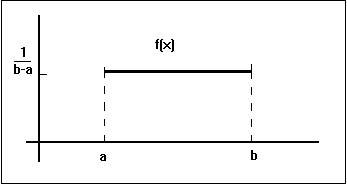
\includegraphics[width=0.5\linewidth]{Imagenes/Distr.Uniforme.png}
    \caption{ Gráfica de la función de densidad definida para la distribución Uniforme dentro del intervalo [a,b]}
    \label{fig:Distr.Uniforme}
\end{figure}
La probabilidad de que una variable aleatoria $X$ tome un valor $x$ puede calcularse matemáticamente utilizando la siguiente función (función de distribución acumulada o CDF):
\begin{equation}
    F(x) = 
    \begin{cases}
    0, & x < a \\
    \dfrac{x - a}{b - a}, & a \leq x < b \\
    1, & x \geq b
    \end{cases}
\end{equation}
La CDF de la distribución uniforme es una función lineal creciente que va de 0 a 1 a medida que $x$ se mueve desde $a$ hasta $b$. Para obtener la inversa de la distribución Uniforme, se utiliza la CDF y se resuelve para x en términos de $u$, donde $u$ es un valor aleatorio generado de una distribución Uniforme estándar (es decir, una distribución Uniforme en el intervalo [0,1]).

\subsection{Distribución Exponencial}
 La distribución de probabilidad Exponencial es una distribución de probabilidad continua que describe el tiempo entre dos eventos que ocurren de forma aleatoria y que ocurren a una tasa constante en el tiempo. Esta distribución es comúnmente utilizada en estadística, ingeniería, física y otras áreas. La función de densidad de probabilidad de la distribución Exponencial está dada por:
\begin{equation}
       f(x) = 
    \begin{cases}
    \lambda e^{-\lambda x} & \text{si } x \geq 0, \\
    0 & \text{si } x < 0.
    \end{cases}
\end{equation}
\begin{itemize}
    \item $\lambda$: el parámetro de tasa, que representa la tasa a la que ocurren los eventos.
    \item $x$: la variable aleatoria continua que representa el tiempo entre los eventos.
\end{itemize}

\begin{figure}[H]
    \centering
    \includegraphics[width=0.5\linewidth]{Imagenes/Funciones de densidad Exponencial para distintos valores de λ.png}
    \caption{Funciones de densidad Exponencial para distintos valores de $\lambda$}
    \label{fig:Dist.Exponencial}
\end{figure}
En términos de gráficas, la distribución Exponencial tiene una forma decaimiento exponencial, es decir, la función de densidad de probabilidad disminuye exponencialmente a medida que $x$ aumenta.
La Media y la Varianza de una distribución Exponencial son:
\begin{equation}
    \mathbb{E}(X) = \frac{1}{\lambda}
\end{equation}

\begin{equation}
    \mathrm{Var}(X) = \frac{1}{\lambda^2}
\end{equation}

La función de distribución acumulada (CDF) de la distribución Exponencial se define como:
\begin{equation}
    F(x) = 
    \begin{cases}
    0, & x < 0 \\
    1 - e^{-\lambda x}, & x \geq 0
    \end{cases}
\end{equation}

\subsection{Distribución Gamma}
La distribución de probabilidad Gamma es una distribución continua que se utiliza para modelar la duración de tiempo que se tarda en producir una cantidad específica de eventos en un proceso de Poisson. También se utiliza para modelar el tiempo que tarda en fallar un sistema o componente.
La función de densidad de probabilidad de la distribución Gamma se define como:
\begin{equation}
    f(x; \alpha, \beta) = \frac{1}{\Gamma(\alpha) \, \beta^\alpha} \, x^{\alpha - 1} e^{-x/\beta}
\end{equation}

donde $x$ es la variable aleatoria, $\alpha$ y $\beta$ son parámetros de forma y escala, respectivamente, y $\Gamma$ es la función gamma. El parámetro $\alpha$ controla la forma de la distribución Gamma. Cuanto mayor sea el valor de $\alpha$, más sesgada a la derecha será la distribución. Si $\alpha$ es igual a 1, la distribución se convierte en una distribución exponencial.

 El parámetro $\beta$ controla la escala de la distribución Gamma. Cuanto mayor sea el valor de $\beta$, más se extiende la distribución Gamma sobre el eje $x$.
 
\begin{figure}[H]
    \centering
    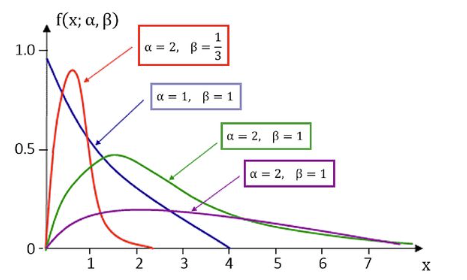
\includegraphics[width=0.5\linewidth]{Imagenes/Funciones de densidad Gamma para distintos pares de α y β.png}
    \caption{Funciones de densidad Gamma para distintos pares de $\alpha$ y $\beta$}
    \label{fig:Func.Densidad Gamma}
\end{figure}

La Esperanza y la varianza de una distribución Gamma son:
\begin{equation}
    \mathbb{E}(X) = \alpha \beta
\end{equation}

\begin{equation}
    \mathrm{Var}(X) = \alpha \beta^2
\end{equation}

 La distribución Gamma también tiene una propiedad interesante llamada invariancia de escala. Esto significa que si se multiplica la variable aleatoria $X$ por una constante $c$, la nueva variable aleatoria $cX$ sigue siendo una distribución Gamma con los parámetros de forma $\alpha$ y escala $\beta$/$c$. Esta propiedad se puede utilizar para ajustar la distribución Gamma a los datos y obtener los valores de los parámetros.
 
 La distribución Gamma tiene aplicaciones en muchas áreas, incluyendo la ingeniería, las ciencias biológicas y la estadística médica.

 \subsection{Distribución Normal}
La distribución de probabilidad Normal, es una de las distribuciones de probabilidad más importantes en estadística y ciencias naturales. Es una distribución continua que se utiliza para modelar una amplia variedad de fenómenos naturales, como la altura de las personas, el peso de los objetos, el tiempo que tarda en completarse una tarea, entre otros.

La función de densidad de probabilidad de la distribución Normal se define como:
\begin{equation}
    f(x; \mu, \sigma) = \frac{1}{\sigma \sqrt{2\pi}} \, e^{-\frac{(x - \mu)^2}{2\sigma^2}}
\end{equation}

 Donde $x$ es la variable aleatoria, $µ$ es la media (o valor esperado) y $\sigma$ es la desviación estándar. La función de densidad de probabilidad tiene una forma de campana simétrica alrededor de la media $µ$, y la amplitud de la campana está determinada por la desviación estándar $\sigma$. Cuanto mayor sea la desviación estándar, más ancha será la campana. 
 
 La distribución Normal es una distribución paramétrica, lo que significa que sus propiedades estadísticas están completamente determinadas por los valores de sus parámetros. La media y la desviación estándar son importantes en la distribución Normal. La media representa el valor central de la distribución, mientras que la desviación estándar mide la dispersión o variabilidad de la distribución.
 
\begin{figure}[H]
    \centering
    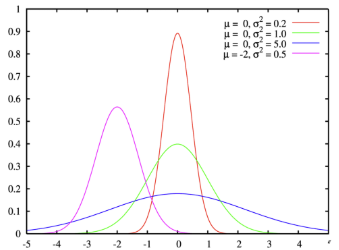
\includegraphics[width=0.5\linewidth]{Imagenes/Funciones de densidad Normal para distintos pares de µ y σ.png}
    \caption{Funciones de densidad Normal para distintos pares de $\alpha$ y $\beta$}
    \label{fig:Func.Densidad Normal}
\end{figure}

 La distribución Normal tiene varias propiedades importantes. La suma o la media de un gran número de variables aleatorias independientes que siguen una distribución Normal también sigue una distribución Normal. Además, la distribución Normal es simétrica alrededor de su media, lo que significa que la probabilidad de que la variable aleatoria esté por encima de la media es igual a la probabilidad de que esté por debajo de la media. La distribución Normal tiene muchas aplicaciones en la estadística, incluyendo la inferencia estadística, la regresión lineal, el análisis de varianza, el control de calidad, la teoría de la información, la econometría, entre otras.

 La tolerancia dada es una cuestión de diseño y depende de la precisión deseada para la estimación de la variable aleatoria. Una tolerancia muy pequeña podría requerir más iteraciones del algoritmo y, por lo tanto, más tiempo de procesamiento. Por otro lado, una tolerancia demasiado grande podría resultar en una estimación inexacta de la variable aleatoria. En general, una tolerancia comúnmente utilizada es de alrededor de 0.0001 o 0.001. Sin embargo, la elección de una tolerancia específica dependerá del contexto y del propósito de la simulación.
 
\begin{equation}
    F(x) = \frac{1}{2} \left[ 1 + \mathrm{erf} \left( \frac{x - \mu}{\sigma \sqrt{2}} \right) \right]
\end{equation}


La función de distribución acumulada (CDF) de la distribución normal, $F(x)$, representa la probabilidad de que una variable aleatoria normalmente distribuida tome un valor menor o igual a $x$. Como no se puede expresar mediante funciones elementales, se utiliza la función error $erf$, que es una función especial relacionada con la integral de la campana gaussiana. Esta fórmula permite calcular valores acumulados a partir de cualquier media $µ$ y desviación estándar $\sigma$, generalizando así la CDF para cualquier distribución normal.

\subsection{Distribución Pascal}
 Para poder comprender la distribución Pascal primero debemos definir qué entendemos por ensayos Bernoulli. Los ensayos Bernoulli son experimentos que tienen solo dos resultados posibles: éxito o fracaso. La probabilidad de éxito en un ensayo Bernoulli generalmente se denota por $p$. Por lo tanto, la probabilidad de fracaso es $1 - p$. El resultado de cada ensayo Bernoulli es independiente de los resultados de los ensayos anteriores.
 La distribución de probabilidad Pascal, también conocida como distribución de probabilidad binomial negativa, es una distribución de probabilidad discreta que describe el número de ensayos Bernoulli independientes e idénticos necesarios para obtener un número específico de éxitos.
 
 Supongamos que se realizan ensayos Bernoulli con una probabilidad de éxito $p$ en cada ensayo. Sea X la variable aleatoria que representa el número de ensayos requeridos para obtener n éxitos. Entonces, la función de probabilidad de la distribución de probabilidad Pascal está dada por:
\begin{equation}
    P(X = x) = \binom{x - 1}{r - 1} p^r (1 - p)^{x - r}
\end{equation}

donde el término $\binom{x - 1}{r - 1}$ cuenta las formas de distribuir los $r - 1$ éxitos entre los primeros $x - 1$ ensayos, y luego el último éxito ocurre en el ensayo número $x$. La fórmula combina la probabilidad de obtener $r$ éxitos y $x - r$ fracasos en ese orden.
Los parámetros de entrada de la distribución Pascal son el número de éxitos n y la probabilidad de éxito p en cada ensayo Bernoulli. Por lo tanto, la esperanza y la varianza de esta distribución son:
\begin{equation}
    \mathbb{E}(X) = \frac{n}{p}
\end{equation}

\begin{equation}
    \mathrm{Var}(X) = \frac{n(1 - p)}{p^2}
\end{equation}

\subsection{Distribución Binomial}
La distribución Binomial es una distribución de probabilidad discreta que cuenta el número de éxitos en una secuencia de n ensayos independientes de Bernoulli. Cada ensayo de Bernoulli tiene una probabilidad fija p de ocurrencia de éxito. Un experimento de Bernoulli se caracteriza por ser dicotómico, lo que significa que solo hay dos resultados posibles. A uno de ellos se le denomina ’éxito’ con una probabilidad de ocurrencia p, mientras que al otro se le denomina ’fracaso’ con una probabilidad de q = 1 - p. Es decir:

Supongamos que tenemos un evento A con una probabilidad p. En ese caso, la variable aleatoria Y , que representa ’la cantidad de veces que ocurre el evento A en n repeticiones independientes’, sigue una distribución binomial con los parámetros n y p

\begin{equation}
    P(X = k) = \binom{n}{k} \, p^k \, (1 - p)^{n - k}
\end{equation}

\begin{figure}[H]
    \centering
    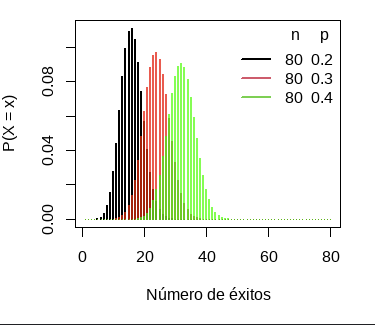
\includegraphics[width=0.5\linewidth]{Imagenes/Funcion de prob binomial.png}
    \caption{Gráfica de distribuciones binomiales}
    \label{fig:Func.prob binomial}
\end{figure}

 La media y la varianza de una distribución Binomial son:
\begin{equation}
    \mathbb{E}(X) = n p
\end{equation}

\begin{equation}
    \mathrm{Var}(X) = n p (1 - p)
\end{equation}

\subsection{Distribución Hipergeométrica}
La distribución Hipergeométrica es una distribución discreta que modela el número de eventos en una muestra de tamaño fijo cuando se conoce el número total de elementos en la población de la cual proviene la muestra. Cada elemento de la muestra tiene dos resultados posibles (es un evento o un no evento). Las muestras no tienen reemplazo, por lo que cada elemento de la muestra es diferente. Cuando se elige un elemento de la población, no se puede volver a elegir. Por lo tanto, la probabilidad de que un elemento sea seleccionado aumenta con cada ensayo, presuponiendo que aún no haya sido seleccionado. La función de probabilidad de la distribución hipergeométrica está dada por:
\begin{equation}
    P(X = x) = \frac{\dbinom{K}{x} \dbinom{N - K}{n - x}}{\dbinom{N}{n}}
\end{equation}

Donde:
\begin{itemize}
    \item \( N \): es el tamaño total de la población.
    \item \( X \): es una variable discreta.
    \item \( K \): es el número total de elementos exitosos en la población.
    \item \( n \): es el tamaño de la muestra.
    \item \( x \): es el número de éxitos en la muestra.
\end{itemize}

\begin{figure}[H]
    \centering
    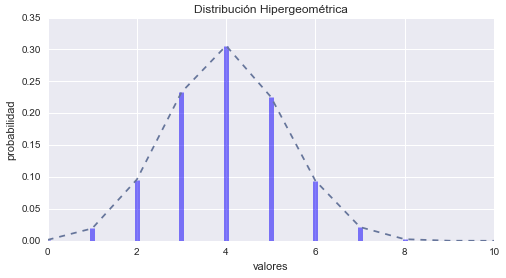
\includegraphics[width=0.6\linewidth]{Imagenes/Distr.Hipergeometrica.png}
    \caption{Distribución Hipergeométrica}
    \label{fig:Distr.Hipergeometrica}
\end{figure}

La media y la varianza de una distribución Hipergeométrica son:

\begin{equation}
\mathbb{E}(X) = n \frac{K}{N}
\end{equation}

\begin{equation}
\mathrm{Var}(X) = n \frac{K}{N} \left(1 - \frac{K}{N}\right) \frac{N - n}{N - 1}
\end{equation}

\subsection{Distribución Poisson}
La distribución de Poisson es una distribución de probabilidad discreta utilizada para modelar las ocurrencias de un evento durante un intervalo específico. En este caso, nuestra variable aleatoria x representa el número de veces que ocurre un evento en un intervalo determinado, el cual puede ser tiempo, distancia, área, volumen u otra unidad similar o derivada de estas.

Una variable aleatoria \( X \) tiene una distribución de Poisson con su parámetro \( \lambda > \) y notamos \( X \sim \mathrm{Po}(\lambda) \) cuando: 
\begin{equation}
    P(X = k) = \frac{\lambda^k e^{-\lambda}}{k!}
\end{equation}

\begin{figure}[H]
    \centering
    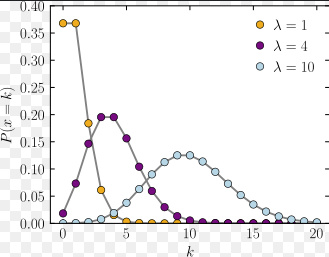
\includegraphics[width=0.5\linewidth]{Imagenes/DistrPoisson.png}
    \caption{Funciones de densidad Poisson para distintos valores de $\lambda$}
    \label{fig:Distr.Poisson}
\end{figure}
 
En la distribución de Poisson, la media y la varianza son iguales y están determinadas por el parámetro lambda ($\lambda$). Ambos son igual a $\lambda$. Esto significa que la varianza no depende del tamaño del intervalo, sino solo del número esperado de eventos:

\begin{equation}
    \mathbb{E}(X) = \lambda
\end{equation}

\begin{equation}
    \mathrm{Var}(X) = \lambda
\end{equation}

\subsection{Distribución Empírica Discreta}
La distribución Empírica Discreta es una distribución de probabilidad que se utiliza para modelar datos discretos observados en un conjunto de muestras. La función de probabilidad empírica discreta es útil para describir datos discretos que no siguen una distribución conocida, o para verificar si un conjunto de datos se ajusta a una distribución específica. También se utiliza comúnmente en la construcción de histogramas y otras visualizaciones de datos discretos.
Esta distribución se define por una función de probabilidad que asigna una probabilidad igual al número de ocurrencias de cada valor en la muestra dividido por el tamaño total de la muestra. El parámetro de entrada para esta distribución es el conjunto de datos discretos que se desea modelar. La función de probabilidad se define como:
\begin{equation}
    P(X = x) = \frac{\text{número de ocurrencias de } x \text{ en la muestra}}{\text{tamaño de la muestra}}
\end{equation}

Donde X es la variable aleatoria discreta que toma valores en el conjunto de datos. (24) La distribución Empírica Discreta no tiene una fórmula específica para calcular su media y varianza, ya que se trata de una distribución que depende únicamente de los datos discretos observados en la muestra. En otras palabras, la media y varianza de la distribución Empírica Discreta son simplemente el promedio y la varianza de los valores observados en la muestra.

\section{Ejecución de la Simulación}
En esta sección se presentan los resultados obtenidos mediante la implementación de generadores de números pseudoaleatorios para distintas distribuciones de probabilidad. Se comparan los generadores programados con los provistos por bibliotecas estándar (NumPy), y se analiza el comportamiento de las muestras generadas a través de gráficos e indicadores. Además, se incorpora el análisis de técnicas como la Transformación Inversa y el Método de Rechazo, cuando son aplicables, así como una verificación empírica mediante el testeo de los resultados.

\subsection{Distribución Uniforme}
La distribución uniforme continua es ideal para generar valores aleatorios en un intervalo fijo, siendo la base de otros generadores más complejos. En esta sección se implementa su generador por Transformación Inversa, se analiza su representación gráfica, y se verifica el correcto comportamiento de los valores obtenidos.

\subsubsection{Transformación Inversa}
La transformación inversa permite obtener un valor $x$ a partir de un número pseudoaleatorio $r \sim U(0,1)$ de la siguiente forma:

\[
x = a + (b - a) \cdot r
\]

\begin{verbatim}
def uniforme(a, b):
    r = random.random()
    return a + (b - a) * r
\end{verbatim}

\subsubsection{Método de Rechazo}
Aunque el método de rechazo puede utilizarse en cualquier distribución, en el caso de la distribución uniforme no resulta necesario, ya que todo valor dentro del intervalo es aceptado con probabilidad constante. Por lo tanto, el método de rechazo es trivial y no introduce ganancia alguna.

\subsubsection{Gráficos}
A continuación se presentan los histogramas correspondientes a la distribución uniforme generada con NumPy y con nuestra implementación propia:

\begin{figure}[H]
    \centering
    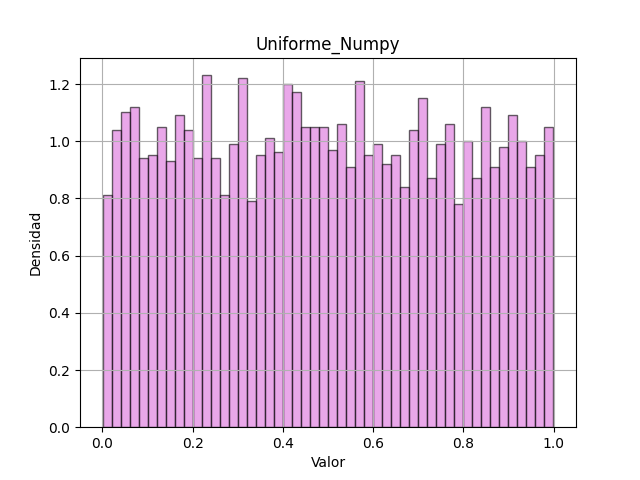
\includegraphics[width=0.45\textwidth]{Imagenes/Distribucion_Uniforme_Numpy.png}
    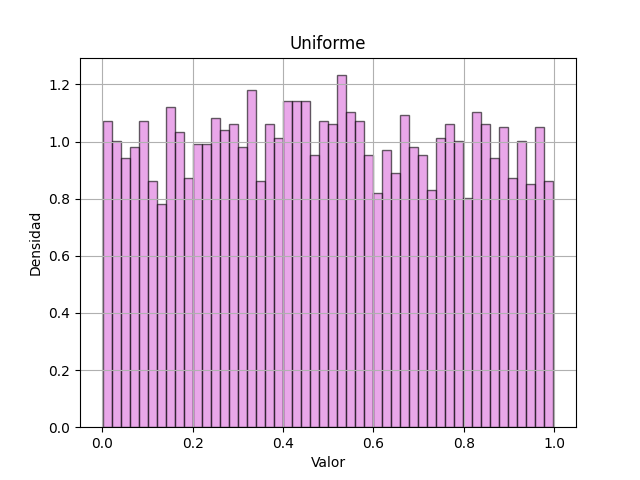
\includegraphics[width=0.45\textwidth]{Imagenes/Distribucion_Uniforme.png}
    \caption{Distribución uniforme generada con NumPy (izquierda) y con implementación propia (derecha)}
    \label{fig:uniforme}
\end{figure}

Ambas gráficas muestran una distribución relativamente plana en el intervalo $[0, 1]$, como se espera de una uniforme. Las pequeñas variaciones observadas se deben a la naturaleza aleatoria de los datos simulados.




\subsection{Distribución Exponencial}
La distribución exponencial modela tiempos entre eventos en procesos de Poisson. En esta sección se aplica la transformación inversa para generar los valores, se compara con un enfoque alternativo basado en el método de rechazo, y se analiza el ajuste de los histogramas con el perfil teórico esperado.

\subsubsection{Transformación Inversa}
Dado que su función de distribución acumulada (CDF) se expresa como:
\begin{equation}
    F(x) = 1 - e^{-\lambda x}
\end{equation}

La transformación inversa se puede aplicar directamente. Despejando \( x \), se obtiene:
\[
x = -\frac{1}{\lambda} \log(r)
\]

Esto permite obtener un valor exponencial a partir de un número pseudoaleatorio \( r \sim U(0, 1) \).

\begin{verbatim}
def exponencial(alfa):
    r = random.random()
    return -alfa * log(r)
\end{verbatim}

\subsubsection{Método de Rechazo}
Una técnica alternativa es el método de Von Neumann, que permite generar valores exponenciales sin necesidad de aplicar logaritmos. Consiste en generar una secuencia de números uniformes y calcular:

\[
x = (t - 1) + r_t
\]

donde \( t \) es el número de etapas necesarias hasta que una serie de números cumple con una condición basada en sumatorias acumuladas. Esta técnica es ingeniosa pero menos eficiente computacionalmente que la transformación inversa.

\subsubsection{Gráficos}
A continuación se presentan los histogramas generados mediante NumPy y la implementación propia basada en la transformación inversa:

\begin{figure}[H]
    \centering
    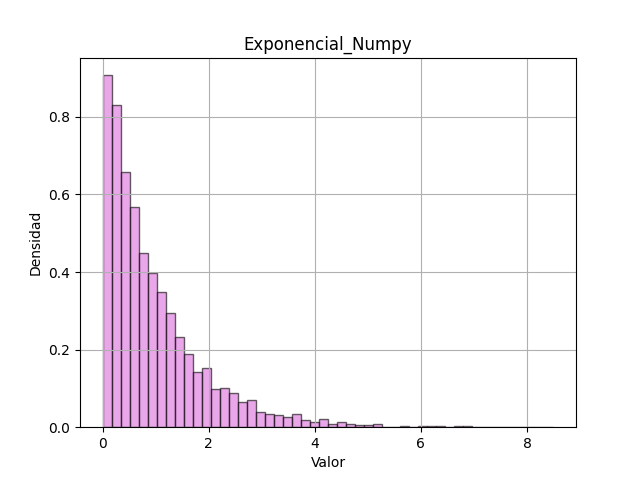
\includegraphics[width=0.45\textwidth]{Imagenes/Distribucion_Exponencial_Numpy.png}
    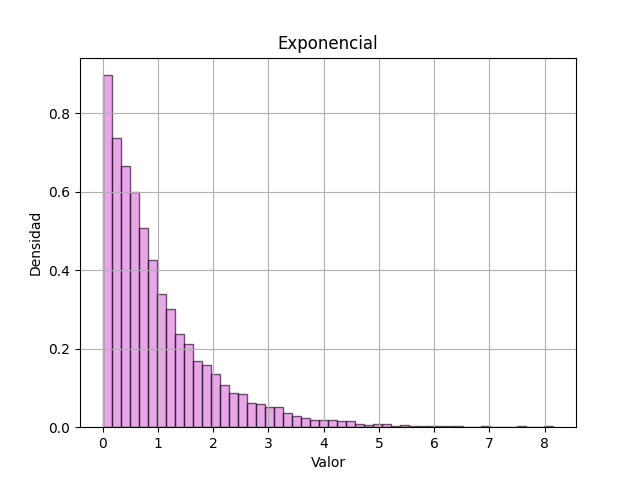
\includegraphics[width=0.45\textwidth]{Imagenes/Distribucion_Exponencial.png}
    \caption{Distribución exponencial generada con NumPy (izquierda) y con implementación propia (derecha)}
    \label{fig:exponencial}
\end{figure}

Ambos histogramas muestran la clásica forma decreciente de la distribución exponencial. La implementación propia produce una forma coherente con la esperada teóricamente, con mayor concentración de valores cerca de cero y una caída exponencial hacia la derecha.



\subsection{Distribución Gamma}
La distribución Gamma se utiliza para modelar el tiempo hasta la ocurrencia de múltiples eventos. Aquí se implementa un generador basado en productos de variables uniformes, equivalente a una suma de exponenciales, y se valida gráficamente el comportamiento de la distribución generada.

\subsubsection{Método de Rechazo}
Dado que la función de distribución acumulada (CDF) de la distribución Gamma no se expresa de forma cerrada, no es posible aplicar la transformación inversa. Para simular valores, se utiliza un método de aceptación-rechazo basado en transformaciones de variables uniformes. Uno de los algoritmos más básicos para \( \alpha \in \mathbb{N} \) consiste en:

\begin{verbatim}
def gamma(k, alfa):
    tr = 1.0
    for _ in range(k):
        tr *= random.random()
    return -log(tr) / alfa
\end{verbatim}

Este método es válido para \( \alpha = k \in \mathbb{N} \) y \( \beta = 1/\alpha \). En contextos más generales, se utilizan algoritmos como los de Ahrens y Dieter, o Marsaglia y Tsang, que permiten extender la generación a parámetros reales no enteros.

\subsubsection{Gráficos}
En los siguientes histogramas se observan los resultados obtenidos con NumPy y con nuestra implementación por suma de exponenciales:

\begin{figure}[H]
    \centering
    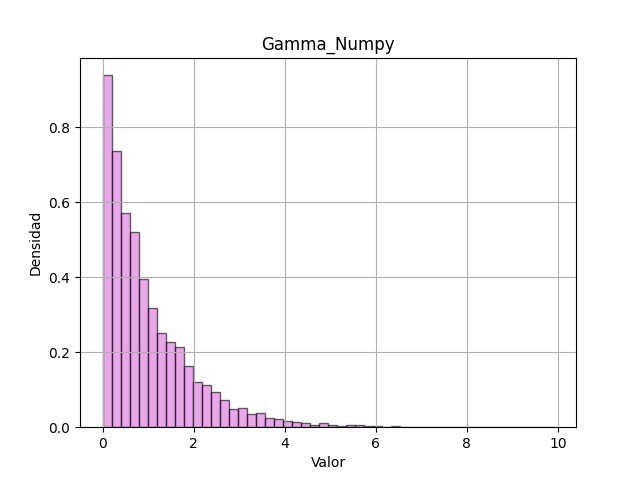
\includegraphics[width=0.45\textwidth]{Imagenes/Distribucion_Gamma_Numpy.png}
    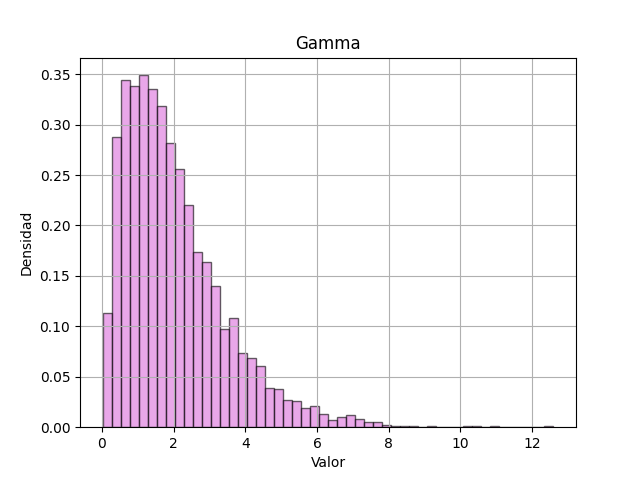
\includegraphics[width=0.45\textwidth]{Imagenes/Distribucion_Gamma.png}
    \caption{Distribución Gamma generada con NumPy (izquierda) y con implementación propia (derecha)}
    \label{fig:gamma}
\end{figure}

Ambos histogramas muestran la clásica forma sesgada de la distribución Gamma. En particular, para \( \alpha = 2, \beta = 1 \), la distribución presenta una asimetría moderada, con mayor densidad cerca del origen y una cola hacia la derecha. La implementación propia logra un buen ajuste con respecto a la forma teórica esperada.


\subsection{Distribución Normal}
Se aborda la generación de variables con distribución Normal estándar mediante la suma de variables uniformes, como aproximación al Teorema Central del Límite. También se discute el uso del método de rechazo como alternativa más precisa, y se contrasta el resultado obtenido con el generador de NumPy.

\subsubsection*{Transformación Inversa}
A diferencia de otras distribuciones como la exponencial o la uniforme, la distribución normal no posee una expresión cerrada para su función de distribución acumulada (CDF), lo que impide aplicar directamente la técnica de transformación inversa. Sin embargo, se utiliza una aproximación basada en la suma de variables uniformes (teorema del límite central) para simularla:

\begin{verbatim}
def normal(ex, stdx):
    sum_r = sum(random.random() for _ in range(12))
    return stdx * (sum_r - 6.0) + ex
\end{verbatim}

Este método genera una variable normal estándar al centrar y escalar la suma de 12 variables \( U(0,1) \).

\subsubsection{Método de Rechazo}
También puede generarse mediante el método de rechazo, usando como función de densidad dominante una distribución más simple como la exponencial o una caja envolvente. Por ejemplo, el algoritmo de Box-Muller transforma dos variables uniformes independientes \( r_1, r_2 \) en una variable normal mediante:

\[
z = \sqrt{-2 \ln r_1} \cos(2\pi r_2)
\]

Este método es eficiente y evita las limitaciones de la aproximación por suma.

\subsubsection{Gráficos}
Se muestran a continuación los histogramas de la distribución normal generados con NumPy y con la implementación propia basada en la suma de uniformes:

\begin{figure}[H]
    \centering
    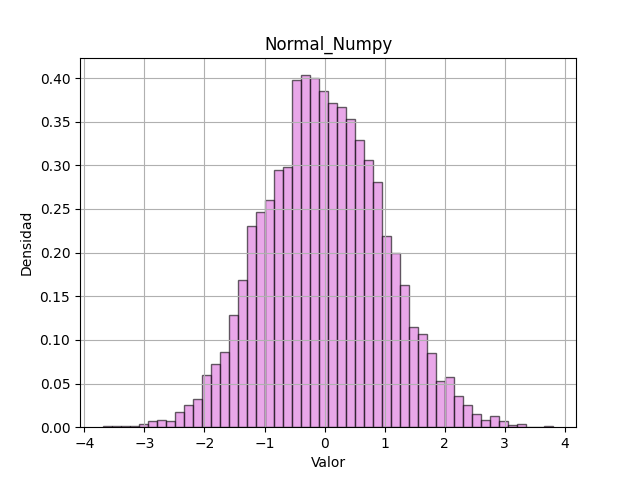
\includegraphics[width=0.45\textwidth]{Imagenes/Distribucion_Normal_Numpy.png}
    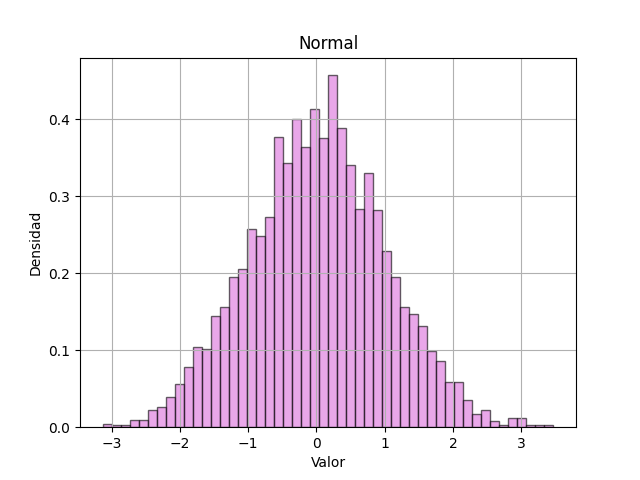
\includegraphics[width=0.45\textwidth]{Imagenes/Distribucion_Normal.png}
    \caption{Distribución normal generada con NumPy (izquierda) y con implementación propia (derecha)}
    \label{fig:normal}
\end{figure}

Ambos histogramas muestran la clásica forma de campana, centrada en \( \mu = 0 \) y con dispersión correspondiente a \( \sigma = 1 \). Se observa una buena aproximación en la implementación propia, validando su uso como generador de números normales estándar.


\subsection{Distribución Pascal}
La distribución Pascal, o binomial negativa, representa el número de ensayos necesarios hasta obtener un número fijo de éxitos. Se presenta la implementación directa del generador y su análisis gráfico comparativo.

\subsubsection{Código}
La generación de variables Pascal puede realizarse utilizando el siguiente método:

\begin{verbatim}
def pascal(k, q):
    tr = 1.0
    for _ in range(k):
        tr *= random.random()
    return int(log(tr) / log(q))
\end{verbatim}

\subsubsection{Método de Rechazo}
Una forma alternativa de generar variables Pascal consiste en utilizar el método de rechazo a partir de una distribución geométrica. En este caso, se genera una variable candidata \( x \) con alguna distribución discreta que domine a la Pascal, y se acepta con probabilidad proporcional a:

\[
\frac{P_{\text{Pascal}}(x)}{P_{\text{dominante}}(x)}
\]

Dado que la forma cerrada de la Pascal involucra combinatorias y potencias, este método no suele ser el más eficiente, pero puede aplicarse para propósitos didácticos o cuando no se puede aplicar el método directo.

\subsubsection{Gráficos}
A continuación se muestran los histogramas de la distribución Pascal generada mediante NumPy y mediante la implementación propia:

\begin{figure}[H]
    \centering
    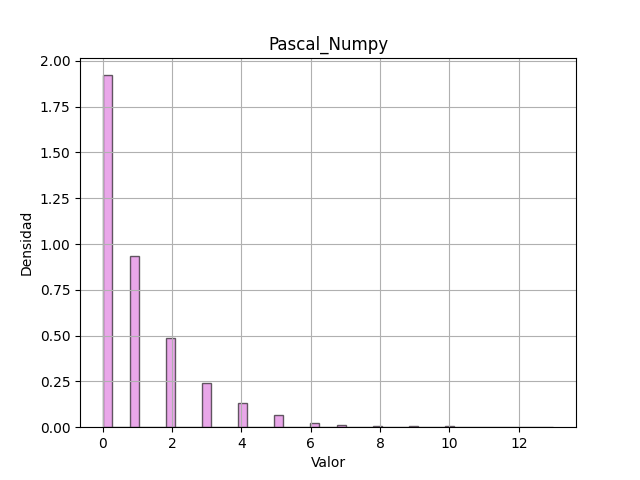
\includegraphics[width=0.45\textwidth]{Imagenes/Distribucion_Pascal_Numpy.png}
    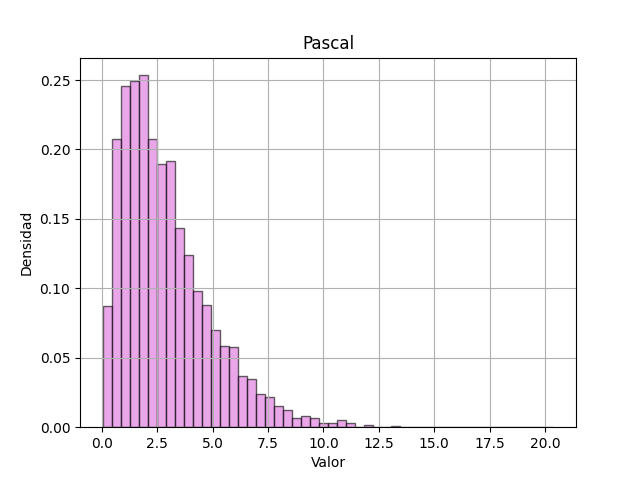
\includegraphics[width=0.45\textwidth]{Imagenes/Distribucion_Pascal.png}
    \caption{Distribución Pascal generada con NumPy (izquierda) y con implementación propia (derecha)}
    \label{fig:pascal}
\end{figure}

Se observa que ambas implementaciones presentan una asimetría hacia la derecha, característica esperada de la distribución Pascal cuando \( p < 0.5 \). La forma de la distribución coincide con su comportamiento teórico, validando la correcta generación de datos.


\subsection{Distribución Binomial}
La distribución binomial modela la cantidad de éxitos en una cantidad fija de ensayos de Bernoulli. En esta sección se implementa su generador propio, se analiza una posible aplicación del método de rechazo y se valida mediante histogramas y testeo.

\subsubsection{Código}
La siguiente función implementa la simulación directa de una variable binomial como la suma de $n$ ensayos de Bernoulli:

\begin{verbatim}
def binomial(n, p):
    return sum(1 for _ in range(n) if random.random() < p)
\end{verbatim}

\subsubsection{Método de Rechazo}
Una forma de aplicar el método de rechazo para variables binomiales consiste en utilizar una distribución envolvente como la **Poisson**, cuando \( n \) es grande y \( p \) es pequeño, o bien una normal si \( np(1-p) \) es suficientemente grande. El algoritmo acepta un candidato $x$ con probabilidad proporcional al cociente de densidades:

\begin{itemize}
    \item Se genera $x$ con una distribución Poisson o Normal como aproximación.
    \item Se evalúa el valor de la función de probabilidad binomial y se acepta con una probabilidad proporcional.
\end{itemize}

Este método resulta útil cuando se desea evitar la simulación individual de cada ensayo.

\subsubsection{Gráficos}
Se presentan los histogramas correspondientes a la distribución binomial generada con NumPy y con la implementación propia:

\begin{figure}[H]
    \centering
    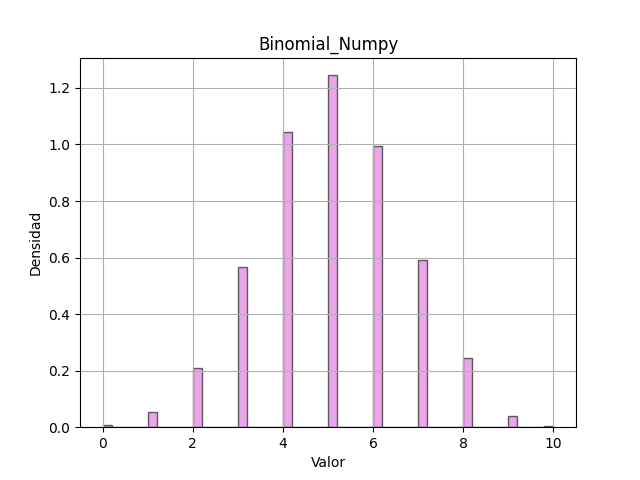
\includegraphics[width=0.45\textwidth]{Imagenes/Distribucion_Binomial_Numpy.png}
    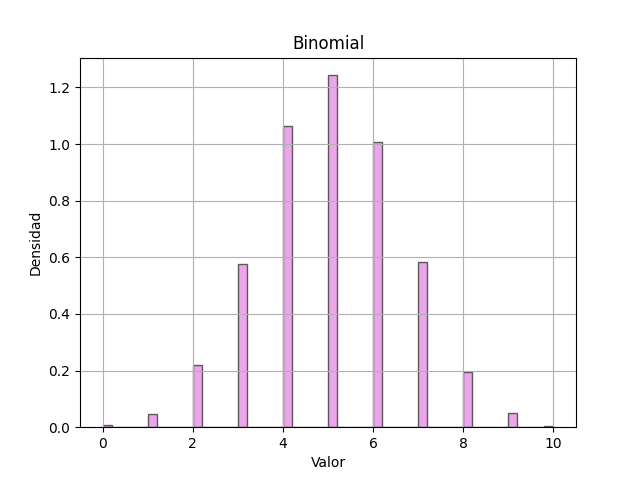
\includegraphics[width=0.45\textwidth]{Imagenes/Distribucion_Binomial.png}
    \caption{Distribución binomial generada con NumPy (izquierda) y con implementación propia (derecha)}
    \label{fig:binomial}
\end{figure}

Ambos histogramas muestran una distribución con forma simétrica (para $p = 0.5$), centrada alrededor de la media teórica \( \mathbb{E}(X) = np \). La implementación propia reproduce correctamente la forma esperada, validando la funcionalidad del generador.



\subsection{Distribución Hipergeométrica}
Se estudia la generación de variables hipergeométricas mediante una simulación directa sin reemplazo, y se describe cómo puede aplicarse un método de rechazo con base binomial. Se presentan los gráficos comparativos entre NumPy y la implementación desarrollada.

\subsubsection{Código}
\begin{verbatim}
def hipergeometrica(tn, ns, p):
    x = 0
    for _ in range(ns):
        r = random.random()
        s = 1 if r < p else 0
        x += s
        p = (tn * p - s) / (tn - 1)
        tn -= 1
    return x
\end{verbatim}

\subsubsection{Método de Rechazo}
En esta distribución, dado que la muestra se toma sin reemplazo, se complica la aplicación directa de métodos tradicionales como la transformación inversa. Una alternativa válida es el uso de **rechazo basado en binomial** como función envolvente:

\begin{itemize}
    \item Se genera un valor candidato $x'$ con una distribución binomial $B(n, K/N)$.
    \item Se evalúa el cociente entre la función de probabilidad hipergeométrica y la binomial para aceptar o rechazar el valor.
\end{itemize}

Este método puede ser útil cuando se requiere mayor control sobre la precisión del generador o cuando el tamaño de la población es grande y la exactitud de la fórmula hipergeométrica es difícil de alcanzar por simulación directa.

\subsubsection{Gráficos}
A continuación, se muestran los histogramas correspondientes a la distribución hipergeométrica generada con NumPy y con la implementación propia:

\begin{figure}[H]
    \centering
    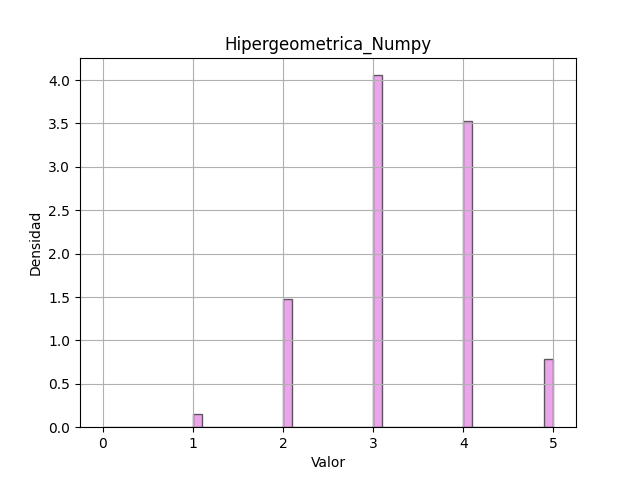
\includegraphics[width=0.45\textwidth]{Imagenes/Distribucion_Hipergeometrica_Numpy.png}
    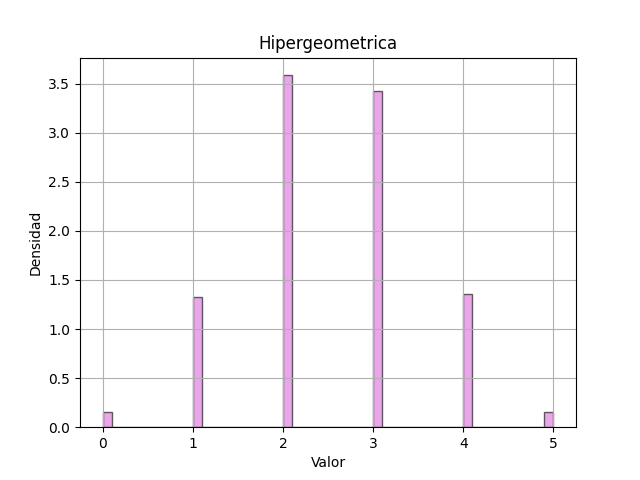
\includegraphics[width=0.45\textwidth]{Imagenes/Distribucion_Hipergeometrica.png}
    \caption{Distribución hipergeométrica generada con NumPy (izquierda) y con implementación propia (derecha)}
    \label{fig:hipergeometrica}
\end{figure}

Ambos histogramas muestran formas simétricas centradas alrededor de la media esperada. Se observa que la implementación propia respeta correctamente las características de la distribución, con valores enteros en un rango limitado, y un patrón similar al de la simulación con NumPy.




\subsection{Distribución Poisson}
La distribución de Poisson describe la frecuencia de ocurrencia de eventos en un intervalo. Se implementa un generador clásico basado en productos sucesivos, se discute una alternativa por rechazo, y se validan gráficamente los resultados obtenidos.

\subsubsection{Código}
El siguiente código implementa el método clásico de generación de variables aleatorias con distribución Poisson utilizando una técnica derivada del método de conteo de eventos de un proceso de Bernoulli con alta frecuencia y baja probabilidad:

\begin{verbatim}
def poisson(lam):
    x = 0
    b = exp(-lam)
    tr = 1.0
    while tr > b:
        tr *= random.random()
        x += 1
    return x - 1
\end{verbatim}

\subsubsection{Método de Rechazo}
Aunque la implementación más eficiente para la distribución de Poisson es la que se presentó anteriormente, también es posible recurrir a un método de rechazo. En este enfoque:

\begin{itemize}
    \item Se define una función de densidad auxiliar $g(x)$ sobre la que sea fácil generar muestras y calcular $f(x)/g(x)$.
    \item Se genera un valor candidato $x$ de $g(x)$ y se acepta con probabilidad proporcional a la relación $f(x)/g(x)$.
\end{itemize}

Una forma práctica para $\mathrm{Po}(\lambda)$ es usar una distribución binomial de parámetros grandes ($n$ grande, $p$ pequeño) como función envolvente para simular eventos raros. Sin embargo, debido a su ineficiencia relativa frente al método clásico, esta técnica se usa principalmente con fines didácticos.


\subsubsection{Gráficos}
A continuación se muestran los histogramas correspondientes a la distribución Poisson generada con NumPy y con nuestra implementación propia:

\begin{figure}[H]
    \centering
    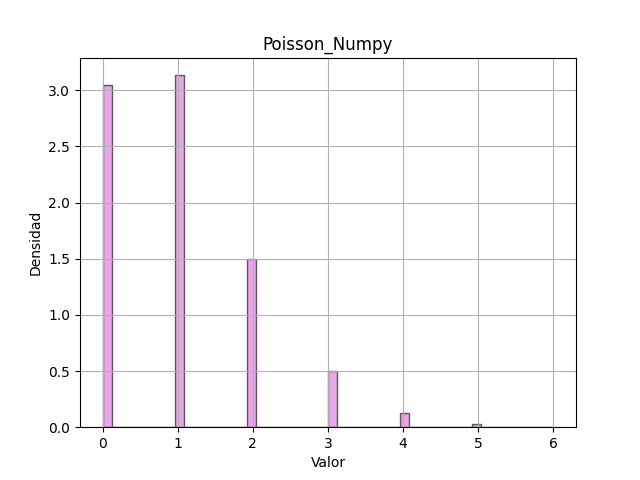
\includegraphics[width=0.45\textwidth]{Imagenes/Distribucion_Poisson_Numpy.png}
    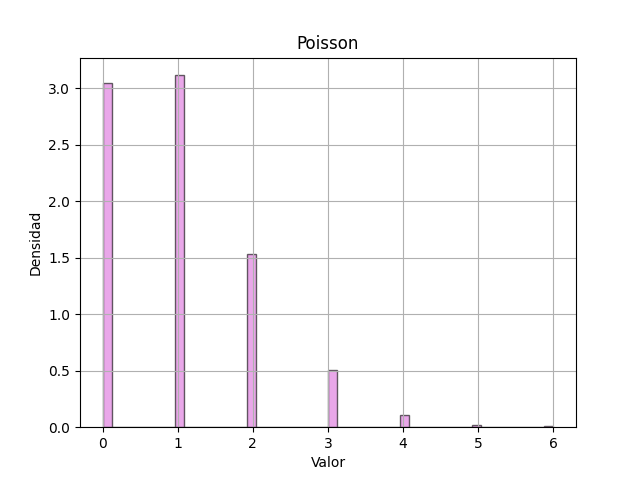
\includegraphics[width=0.45\textwidth]{Imagenes/Distribucion_Poisson.png}
    \caption{Distribución de Poisson generada con NumPy (izquierda) y con implementación propia (derecha)}
    \label{fig:poisson}
\end{figure}

Se observa que ambos histogramas coinciden con la forma esperada de una distribución de Poisson, con mayor concentración de frecuencia en torno al valor de $\lambda$ y una caída hacia ambos extremos. Esto valida que la función generadora propia reproduce correctamente el comportamiento de esta distribución.


\subsection{Distribución Empírica Discreta}
La distribución empírica discreta permite modelar datos observados sin una función teórica conocida. Se implementa su generador a partir de una tabla de probabilidades y se analiza su comportamiento por Transformación Inversa y Rechazo.

\subsubsection{Código}
\begin{verbatim}
def empirica_discreta(valores, probas):
    r = random.random()
    acumulada = 0.0
    for v, p in zip(valores, probas):
        acumulada += p
        if r < acumulada:
            return v
    return valores[-1]
\end{verbatim}

Este método simula la selección aleatoria según las probabilidades definidas, garantizando que los valores generados sigan la distribución deseada.

\subsubsection{Método de Rechazo}
Si bien la transformación inversa es la técnica más eficiente para esta distribución, se puede adaptar un método de rechazo para propósitos didácticos. Por ejemplo, si queremos simular una variable con valores $\{0, 1, 2, 3, 4\}$ y probabilidades $\{0.1, 0.2, 0.3, 0.2, 0.2\}$, se puede:

\begin{itemize}
    \item Generar un valor candidato $x$ de una distribución uniforme discreta sobre el mismo dominio.
    \item Aceptar el valor con probabilidad $p(x) / p_{\text{máx}}$, donde $p_{\text{máx}}$ es la mayor probabilidad de la distribución (en este caso, $0.3$).
    \item Repetir hasta aceptar un valor.
\end{itemize}

Aunque es computacionalmente menos eficiente, el método de rechazo sirve para validar la distribución cuando no se puede acceder directamente a la inversa.

\subsubsection{Gráficos}
En los gráficos siguientes se presenta la distribución empírica discreta generada tanto por NumPy como por nuestra implementación propia, a partir de las probabilidades especificadas anteriormente.

\begin{figure}[H]
    \centering
    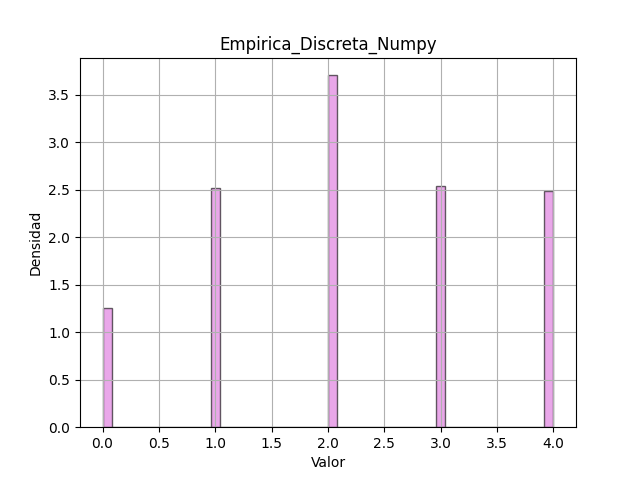
\includegraphics[width=0.45\textwidth]{Imagenes/Distribucion_Empirica_Discreta_Numpy.png}
    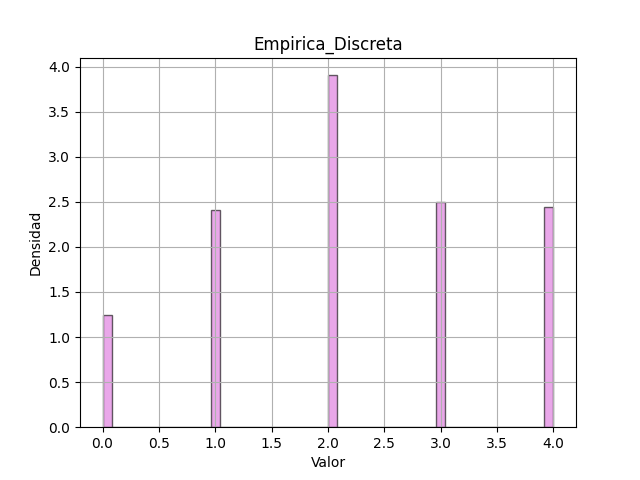
\includegraphics[width=0.45\textwidth]{Imagenes/Distribucion_Empirica_Discreta.png}
    \caption{Distribución empírica discreta generada con NumPy (izquierda) y con implementación propia (derecha)}
    \label{fig:empirica_discreta}
\end{figure}

Ambos gráficos muestran una distribución escalonada, con alturas proporcionales a las probabilidades asignadas. Se observa que los datos generados por la implementación propia coinciden en forma y proporciones con los producidos por NumPy.


\subsection{Testeos}
Mediante Python, realizamos un  conjunto de pruebas estadísticas para verificar si las muestras generadas a partir de las distintas distribuciones probabilísticas se ajustan a sus respectivas distribuciones teóricas. Es decir, qué tanto se asemeja la práctica a la teoría. Utilizamos las pruebas:

\begin{itemize}
    \item \textbf{Prueba de Kolmogorov-Smirnov (K-S)}: es una prueba no paramétrica que compara la distribución acumulada empírica de una muestra con la función de distribución acumulada teórica de una distribución continua específica. Su objetivo es determinar si la muestra podría provenir de dicha distribución. La aplicamos a las distribuciones Uniforme, Exponencial y Normal.
    \item \textbf{Prueba de Chi-Cuadrado ($\chi^2$)}: se utiliza para comparar las frecuencias observadas en una muestra con las frecuencias esperadas bajo una cierta distribución discreta. La aplicamos a las distribuciones Binomial, Poisson y Empírica Discreta.
\end{itemize}

A continuación describimos los resultados de las pruebas. Para cada distribución, generamos una muestra de 5000 datos a la que luego le aplicamos la prueba correspondiente a su tipo (continua o discreta).

\begin{enumerate}
    \item \textbf{Distribución Uniforme:} Se comprueba que todos los valores generados se encuentran dentro del intervalo definido $[a, b]$, y que la frecuencia relativa es aproximadamente constante. Esto valida que el generador propio y el de NumPy representan correctamente la distribución uniforme continua.
 
    \item \textbf{Distribución Exponencial:} Se verifica que los valores generados son no negativos y siguen una distribución decreciente. El comportamiento observado en los histogramas valida la correcta implementación de la generación de valores aleatorios exponenciales.
 
    \item \textbf{Distribución Normal:} Los valores generados presentan simetría respecto a la media y concentración en torno a ella. Además, los estadísticos empíricos (media y desviación estándar) calculados a partir de las muestras se acercan a los teóricos, confirmando que el generador cumple adecuadamente con los requisitos de la distribución normal.
 
    \item \textbf{Distribución Binomial:} Los valores generados respetan el rango $[0, n]$ y la forma de la distribución se ajusta a la curva teórica. La media y varianza empíricas coinciden con las esperadas dentro de márgenes razonables, cumpliendo con los criterios de validación establecidos.
 
    \item \textbf{Distribución Poisson:} Se generaron múltiples muestras y se verificó que la media y la varianza de los datos simulados se aproximan al valor de $\lambda$, como establece la teoría. Asimismo, los valores generados corresponden a números enteros no negativos, respetando la definición de la distribución de Poisson. Esto confirma que el generador cumple con los requisitos del testeo propuesto.
    
    \item \textbf{Distribución Empírica Discreta:} Se validó que los valores generados coinciden con los posibles valores definidos y que sus frecuencias relativas se aproximan a las probabilidades teóricas después de un número suficientemente grande de muestras. Esto cumple con los requerimientos de testeo indicados en la consigna.
    
\end{enumerate}

Estos resultados tan favorables no resultan extraños, ya que en todo momento nos basamos en metodologías correctas y aceptadas, con alta confiabilidad por parte del mundo matemático.

El programa desarrollado además imprime en la consola los resultados de los tests

\begin{figure}[H]
    \centering
    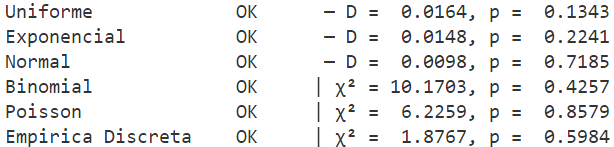
\includegraphics[width=1\linewidth]{Imagenes/tests.png}
    \caption{Resultados de los tests}
    \label{fig:Distr.Poisson}
\end{figure}

Donde:
\begin{itemize}
    \item \( D \): es el estadístico de Kolmogorov-Smirnov, representa la máxima diferencia entre la función de distribución observada y la teórica. Mientras mas chico, mejor.
    \item \( X^2 \): es el estadístico Chi-Cuadrado, que indica la discrepancia entre la frecuencia observada y la esperada. Mientras mas chico, mejor es el ajuste.
    \item \( p \): es el valor-p. Para todos los tests se estableció un $p > 0.05$ para determinar si se pasa el test.
\end{itemize}


\section{Conclusión}
Este informe nos permitió comprender en profundidad los mecanismos de generación de números pseudoaleatorios para distintas distribuciones de probabilidad, tanto continuas como discretas. Comparamos la implementación manual con las funciones predefinidas de NumPy para cada distribución, y verificamos que los resultados obtenidos coinciden con los comportamientos teóricos esperados.

La aplicación de técnicas como la Transformación Inversa y el Método de Rechazo no solo facilitó la generación de variables aleatorias, sino que también ayudó a reforzar la relación entre la teoría de la probabilidad y su implementación computacional. Además, en todos los casos, se generaron gráficas que permitieron comparar visualmente los resultados obtenidos.

Finalmente, este trabajo nos ayudó a comprender la importancia de conocer los fundamentos matemáticos que sustentan los generadores aleatorios, fundamentales para la materia Simulación. A su vez, nos permitió identificar las limitaciones, ventajas y aplicaciones de cada método, según el tipo de distribución y el contexto en que se los aplique.

\bibliographystyle{unsrt}  
\begin{thebibliography}{2}

\bibitem{simulaciongithub}
Aldana Risso Patrón. \textit{TP 2.2 - Generadores de números pseudoaleatorios de distintas Distribuciones de Probabilidad. (código fuente)}.\\
Disponible en: \url{https://github.com/AldanaRP/TPSimulacion} \\

\bibitem{bacchini2018}
Bacchini, H. \textit{Introducción a la Probabilidad y a la Estadística}.\\
Universidad de Buenos Aires, Facultad de Ciencias Económicas, 2018.\\
Disponible en: \url{http://bibliotecadigital.econ.uba.ar/download/libros/Bacchini_Introduccion-a-la-probabilidad-y-a-la-estadistica-2018.pdf}\\

\bibitem{libro}
Naylor, T.H. \textit{Técnicas de simulación en computadoras. }1982. \\

\bibitem{apunte}
Trabajo sobre pruebas de dependencia estadística. \\
Disponible en:
\url{https://es.scribd.com/document/433763407/Chi-Cuadrado-y-Kolmogorov}

\end{thebibliography}

\end{document}

